%TODO: This needs restructuring.
%NAME: Συμπληρωματικές γωνίες.svg
\documentclass{standalone}

\usepackage{tikz}
\usepackage{graphicx}
\usepackage{amssymb}
\usetikzlibrary{arrows.meta,decorations.markings}

\usetikzlibrary{calc}
\definecolor{Blue}{RGB}{13,93,184}

\def\StartAngle{0}
\def\EndAngle{\StartAngle + 61.7419704}
\def\PLength{0.80622577483}
\def\Px{1}
\def\Py{0}
\def\PPx{0}
\def\PPy{1}
\def\Scale{0.04}

\def\Cx{0.43}
\def\Cy{0.8}
\def\CLength{0.908240056}

\def\AngleLen{0.15}

\begin{document}
\scalebox{5.0}{
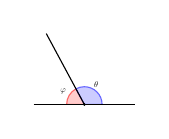
\begin{tikzpicture}[scale=1.5]
\clip(-0.05, -0.05) rectangle (2 * \Cx + 0.05, 0.75 * \Cy + 0.05);

\node (p) at (\Px, \Py) {};
\node (pp) at (\PPx, \PPy) {};

\filldraw[fill=red!20!white,draw=red!60!white] (\Cx, 0) -- (\Cx - \AngleLen, 0) arc (180:(180 - 61.7419704):\AngleLen) -- (\Cx,0);
\filldraw[fill=blue!20!white,draw=blue!60!white] (\Cx, 0) -- (\Cx + \AngleLen, 0) arc (0:(180 - 61.7419704):\AngleLen) -- (\Cx,0);

\draw (0, 0) -- (2 * \Cx, 0);

\draw (\Cx, 0) -- (0.25 * \Cx, \Cy * 0.75);

\node at (0.53, 0.172) {\scalebox{0.3}{$\theta$}};
\node at (0.25, 0.11) {\scalebox{0.3}{$\varphi$}};

\node[circle, fill=black, scale=0.12] at (\Cx, 0) {};
\end{tikzpicture}}
\end{document}   

